
\section{Durchführung}
\label{sec:Durchführung}
\subsection{Experimenteller Aufbau}
\begin{figure}
\caption{Aufbau einer Wärmepumpe\cite{V206}}
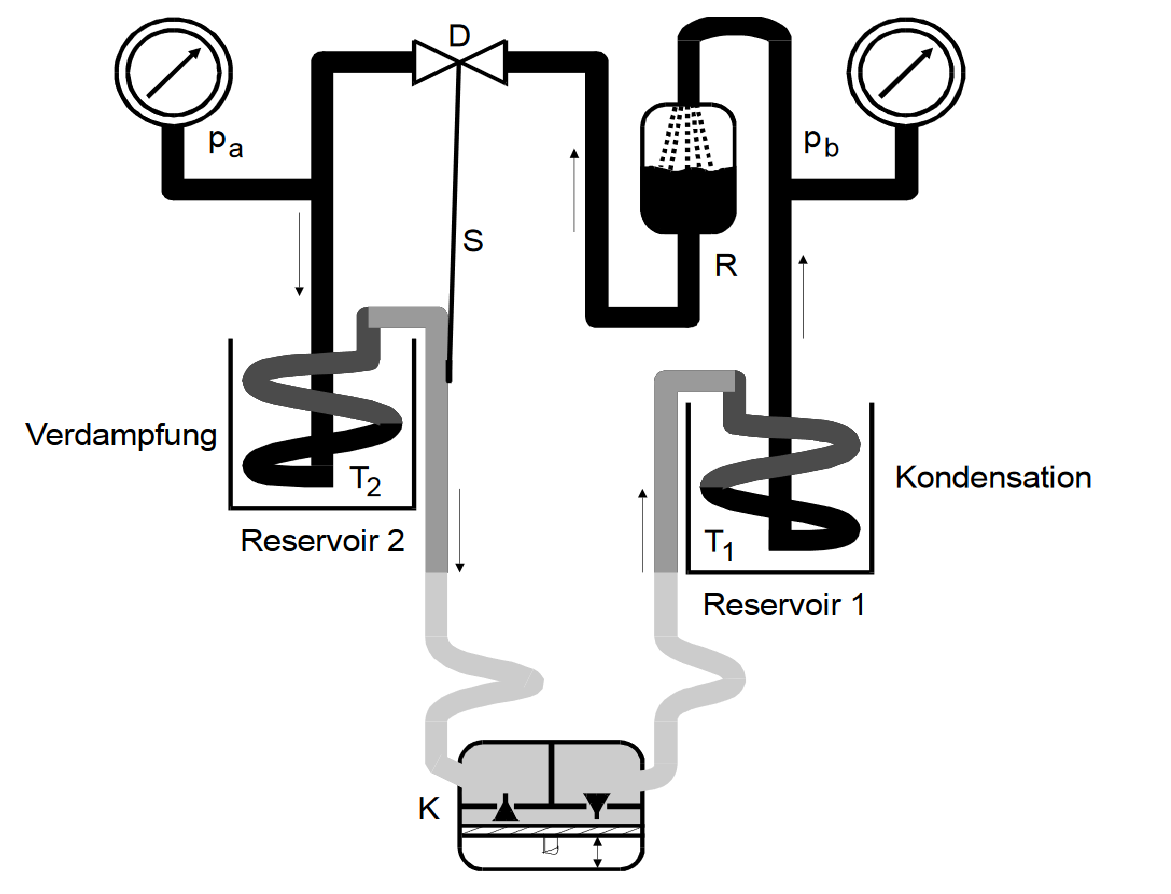
\includegraphics[scale=0.5]{content/images/aufbau.eps}
\label{fig:abb1}
\end{figure}
\noindent Als Transportgas wird ein reales Gas verwendet (hier $Cl_.{2}F_.{2}C$), das bei $T_.{1}$ und $p_.{b}$ flüssig und bei $T_.{2}$ und $p_.{a}$ gasförmig ist.
Der Kompressor $K$ sorgt für einen Kreislauf des Mediums in der Pumpe.\newline
Zwischen den beiden Wärmereservoirs liegt das Drosselventil $D$
an dem sich der Druckunterschied $p_.{b}-p_.{a}$ aufbaut.\newline
Das flüssige Medium verdampft, nachdem es $D$ passiert, im wärmeabegebenden Reservoir 2 und entzieht ihm die Verdampfungswärme $L$.
Anschließend wird es im Kompressor adiabatisch komprimiert, sodass es im Reservoir 1 wieder verflüssigt und dabei die Kondensationswärme $L$ an dieses abgibt.
\subsection{Durchführung}
Die beiden Reservoirs werden mit einer exakten Menge Wasser befüllt.\newline
Nach dem Starten der Pumpe werden einmal pro Minute die Werte für $T_.{1}$, $T_.{2}$, $p_.{a}$, $p_.{b}$ und $P_.{m}$ gemessen